\subsection{part c}
For transfer function we use common architecture.
\begin{figure}[H]
    \caption{Architecture}
    \centering
    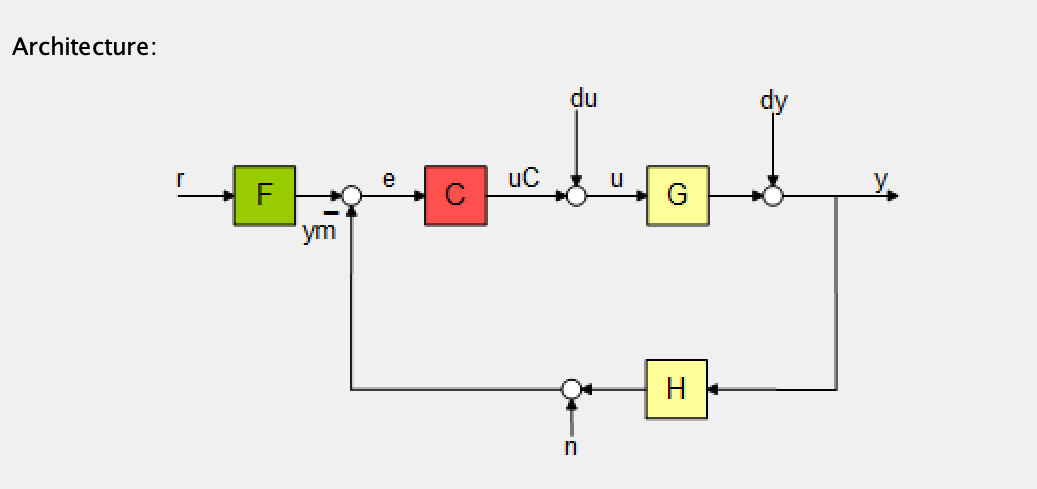
\includegraphics[width=12cm]{../Figure/Q1/Q1_c/architecture.png}
\end{figure}
\begin{itemize}
    \item r to y refrence
    $$
    \dfrac{y}{r} = \dfrac{C(s)G(s)}{1+C(s)G(s)}
    $$
    \begin{figure}[H]
        \caption{r to y bode magnitude}
        \centering
        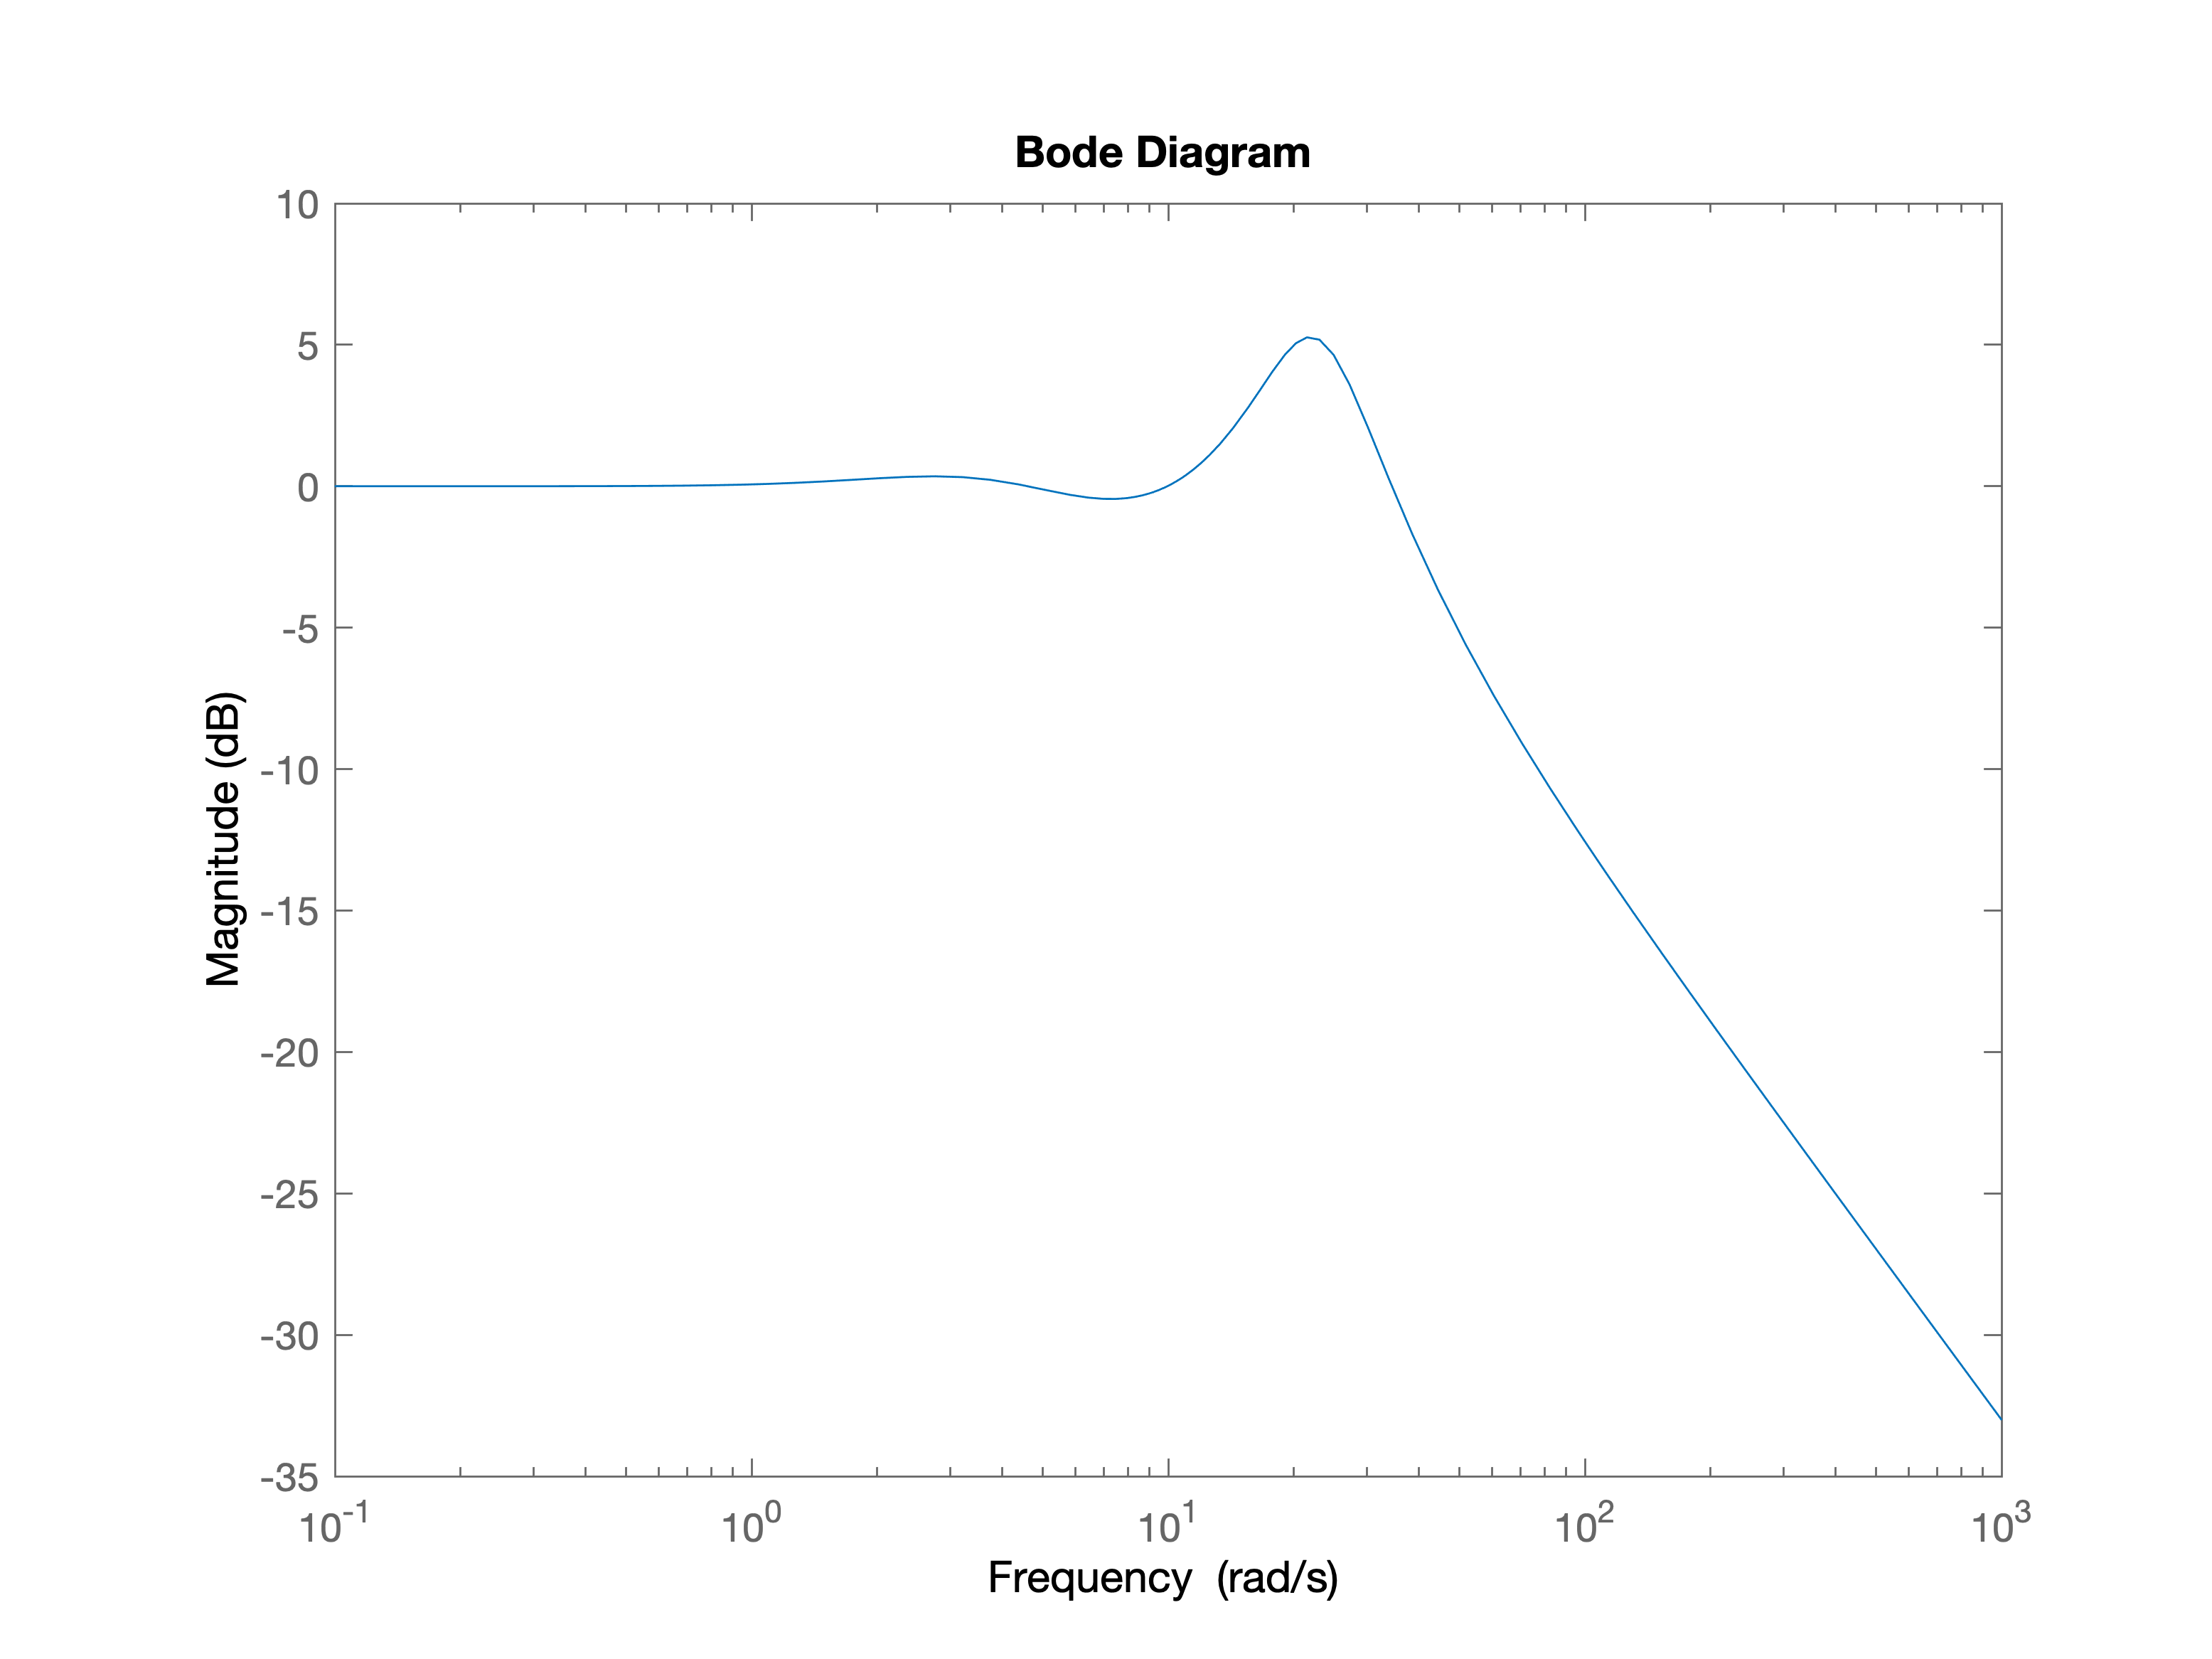
\includegraphics[width=12cm]{../Figure/Q1/Q1_c/bode_r2y.png}
    \end{figure}
    System has a good performance at high frequency but not good performance at low frequency.
    \item du to y distubance
    $$
    \dfrac{y}{du} = \dfrac{G(s)}{1+C(s)G(s)}
    $$
    \begin{figure}[H]
        \caption{du to y bode magnitude}
        \centering
        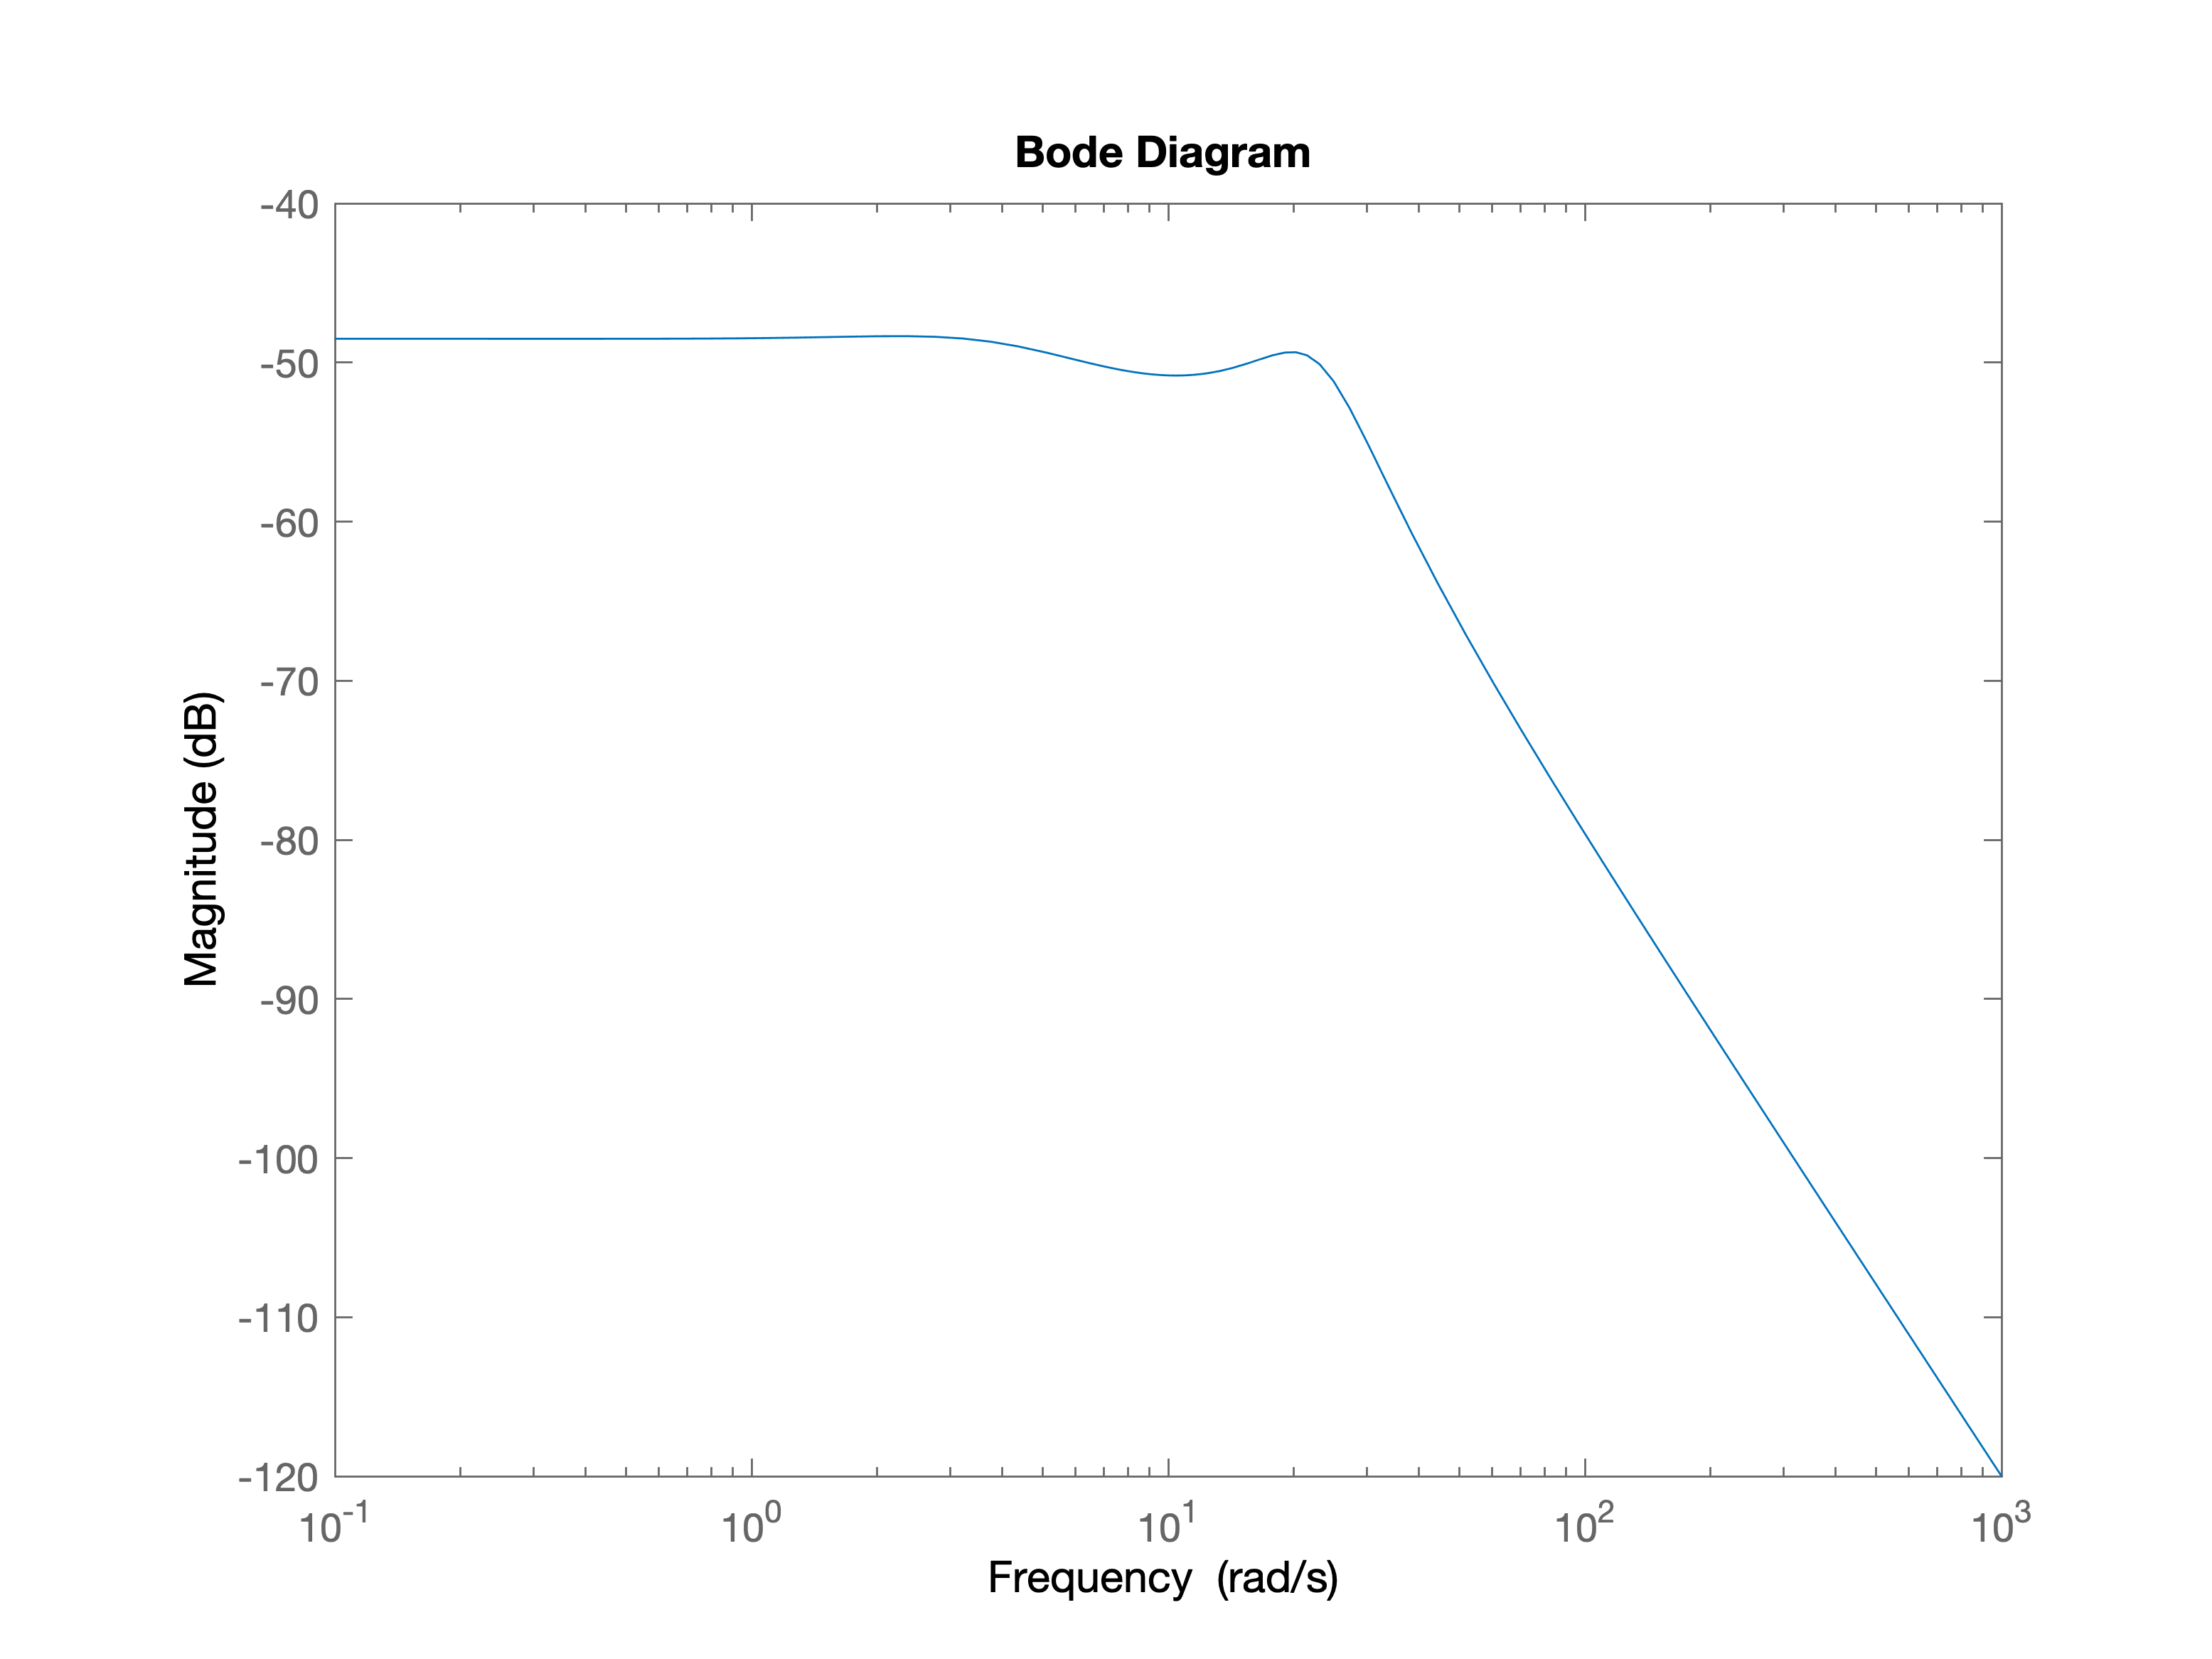
\includegraphics[width=12cm]{../Figure/Q1/Q1_c/bode_du2y.png}
    \end{figure}
    System has a better performance at high frequency but pretty good performance at low frequency.
    \item dy to y distubance
    $$
    \dfrac{y}{dy} = \dfrac{1)}{C(s)G(s)}
    $$
    \begin{figure}[H]
        \caption{dy to y bode magnitude}
        \centering
        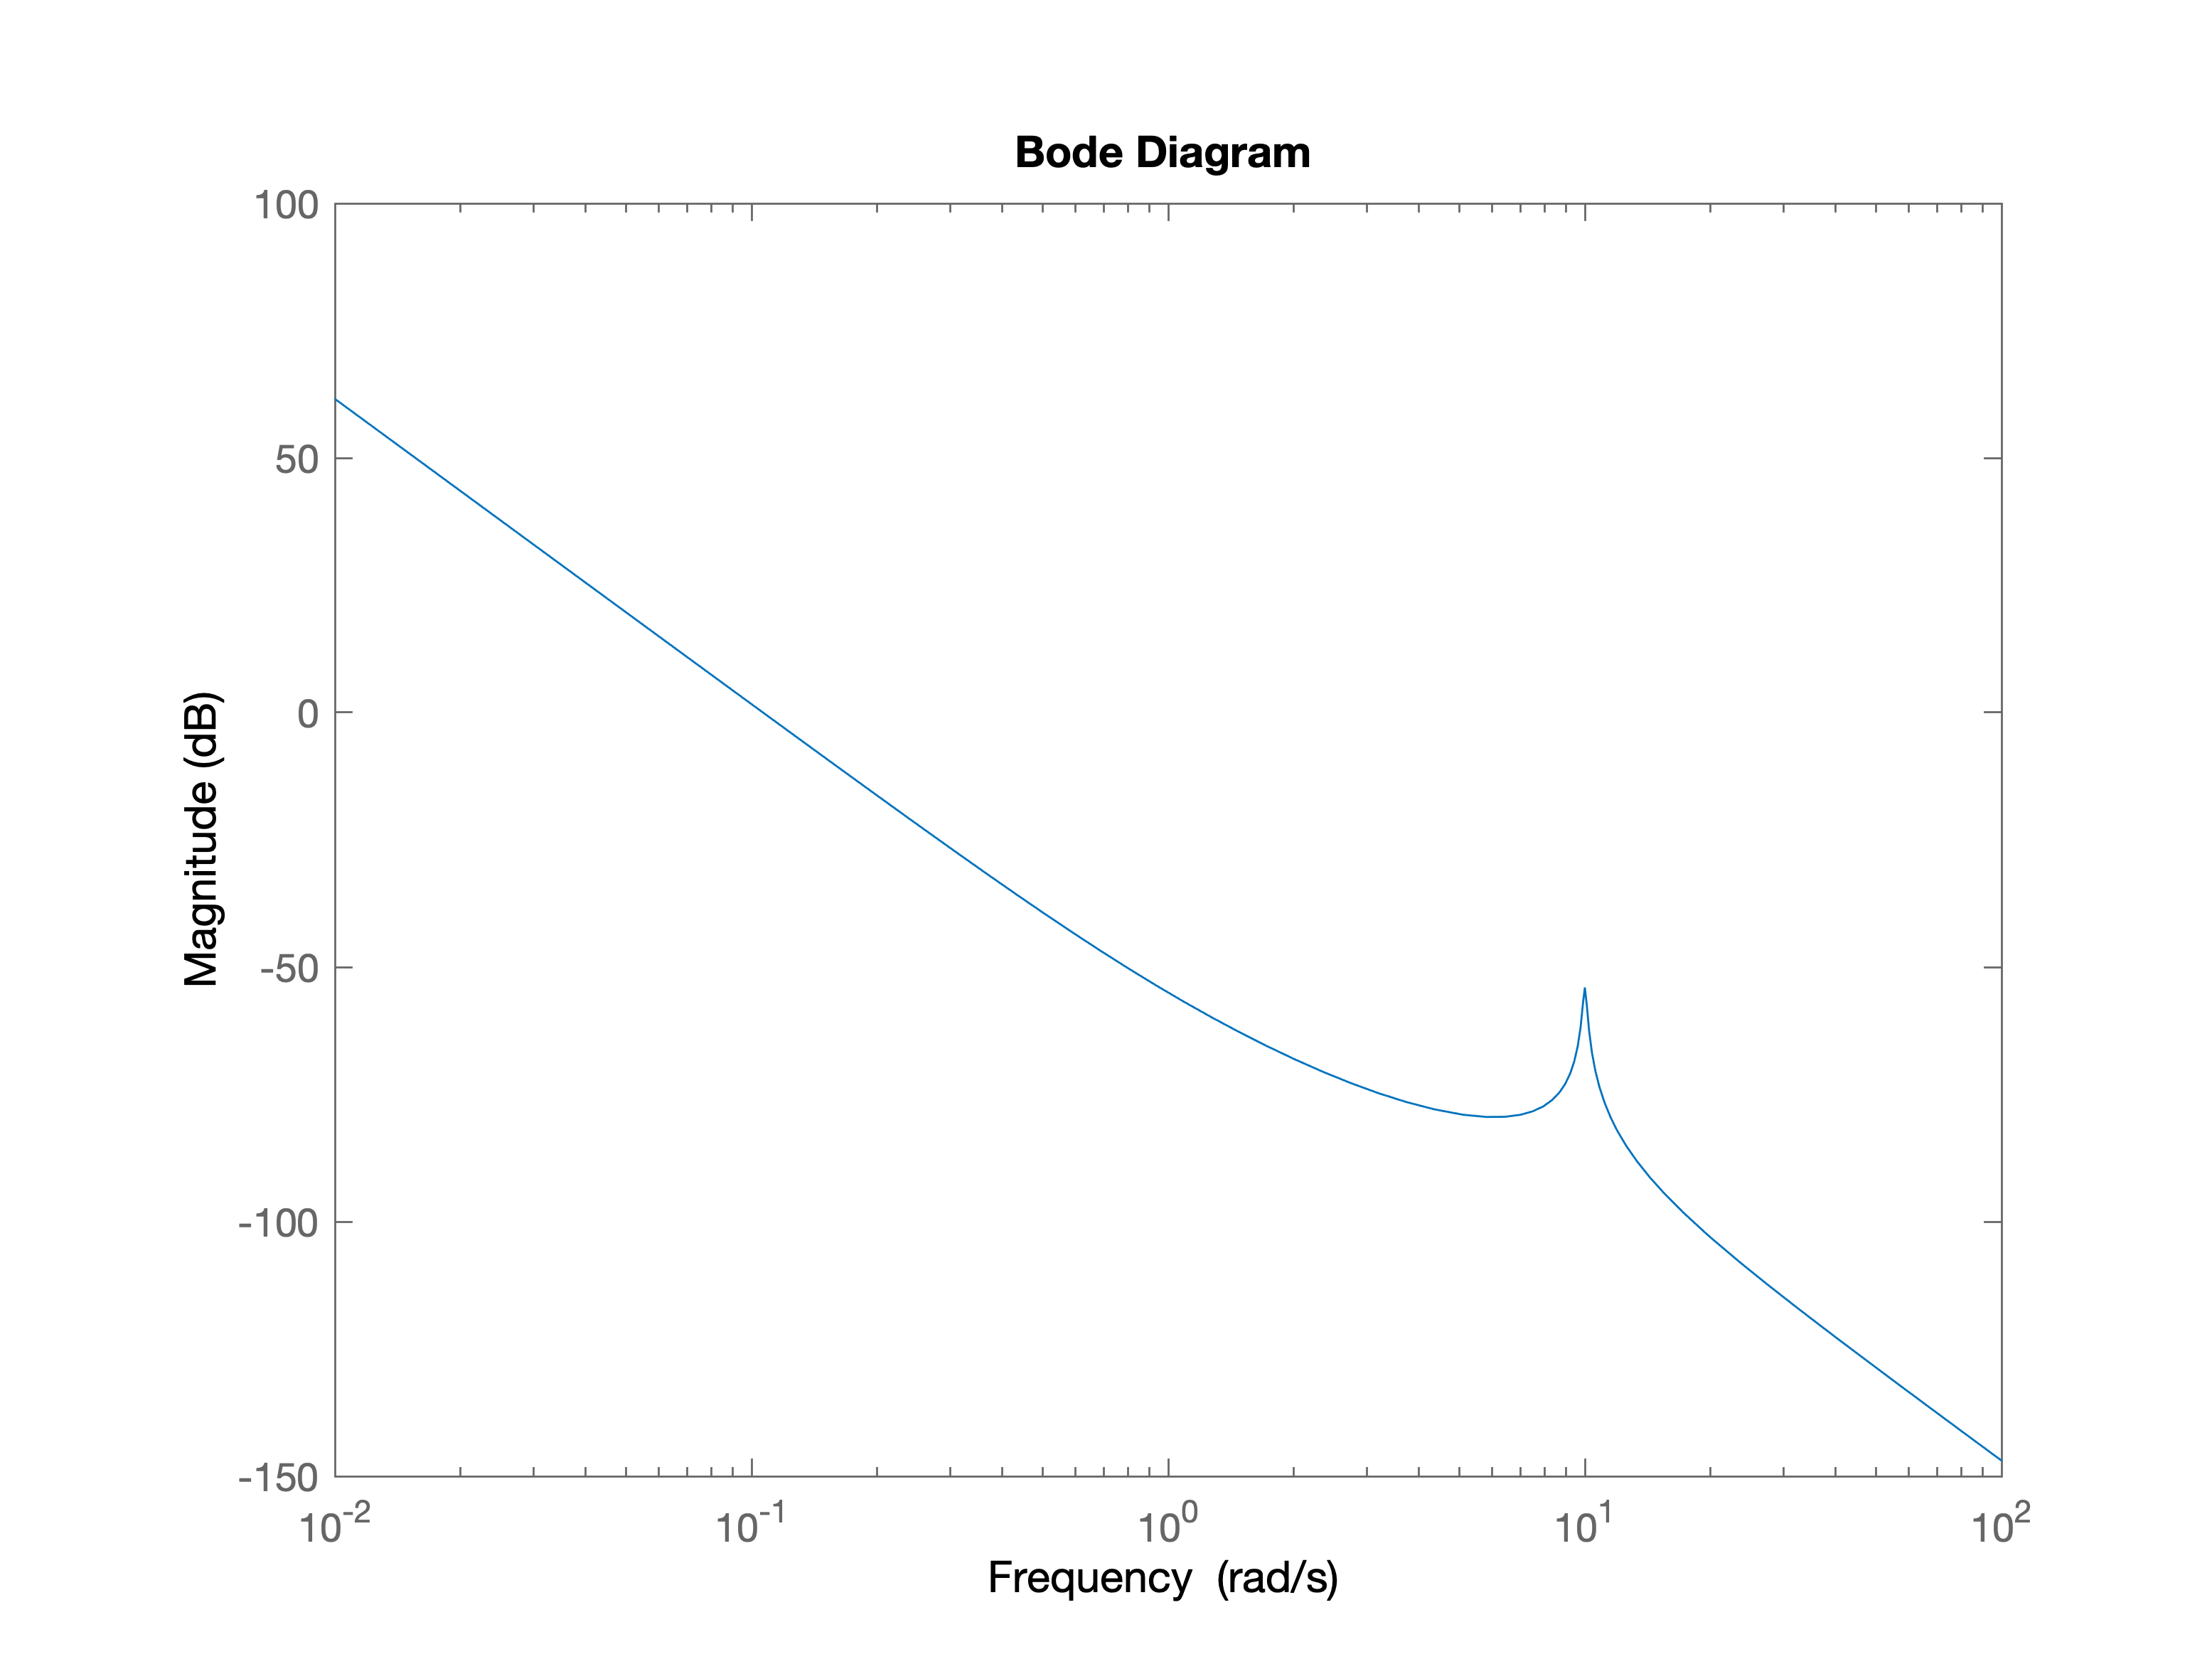
\includegraphics[width=12cm]{../Figure/Q1/Q1_c/bode_dy2y.png}
    \end{figure}
    System has a good performance at high frequency but very bad performance at low frequency.
    \item n to y noise
    $$
    \dfrac{y}{du} = \dfrac{-C(s)G(s)}{1+C(s)G(s)}
    $$
    \begin{figure}[H]
        \caption{n to y bode magnitude}
        \centering
        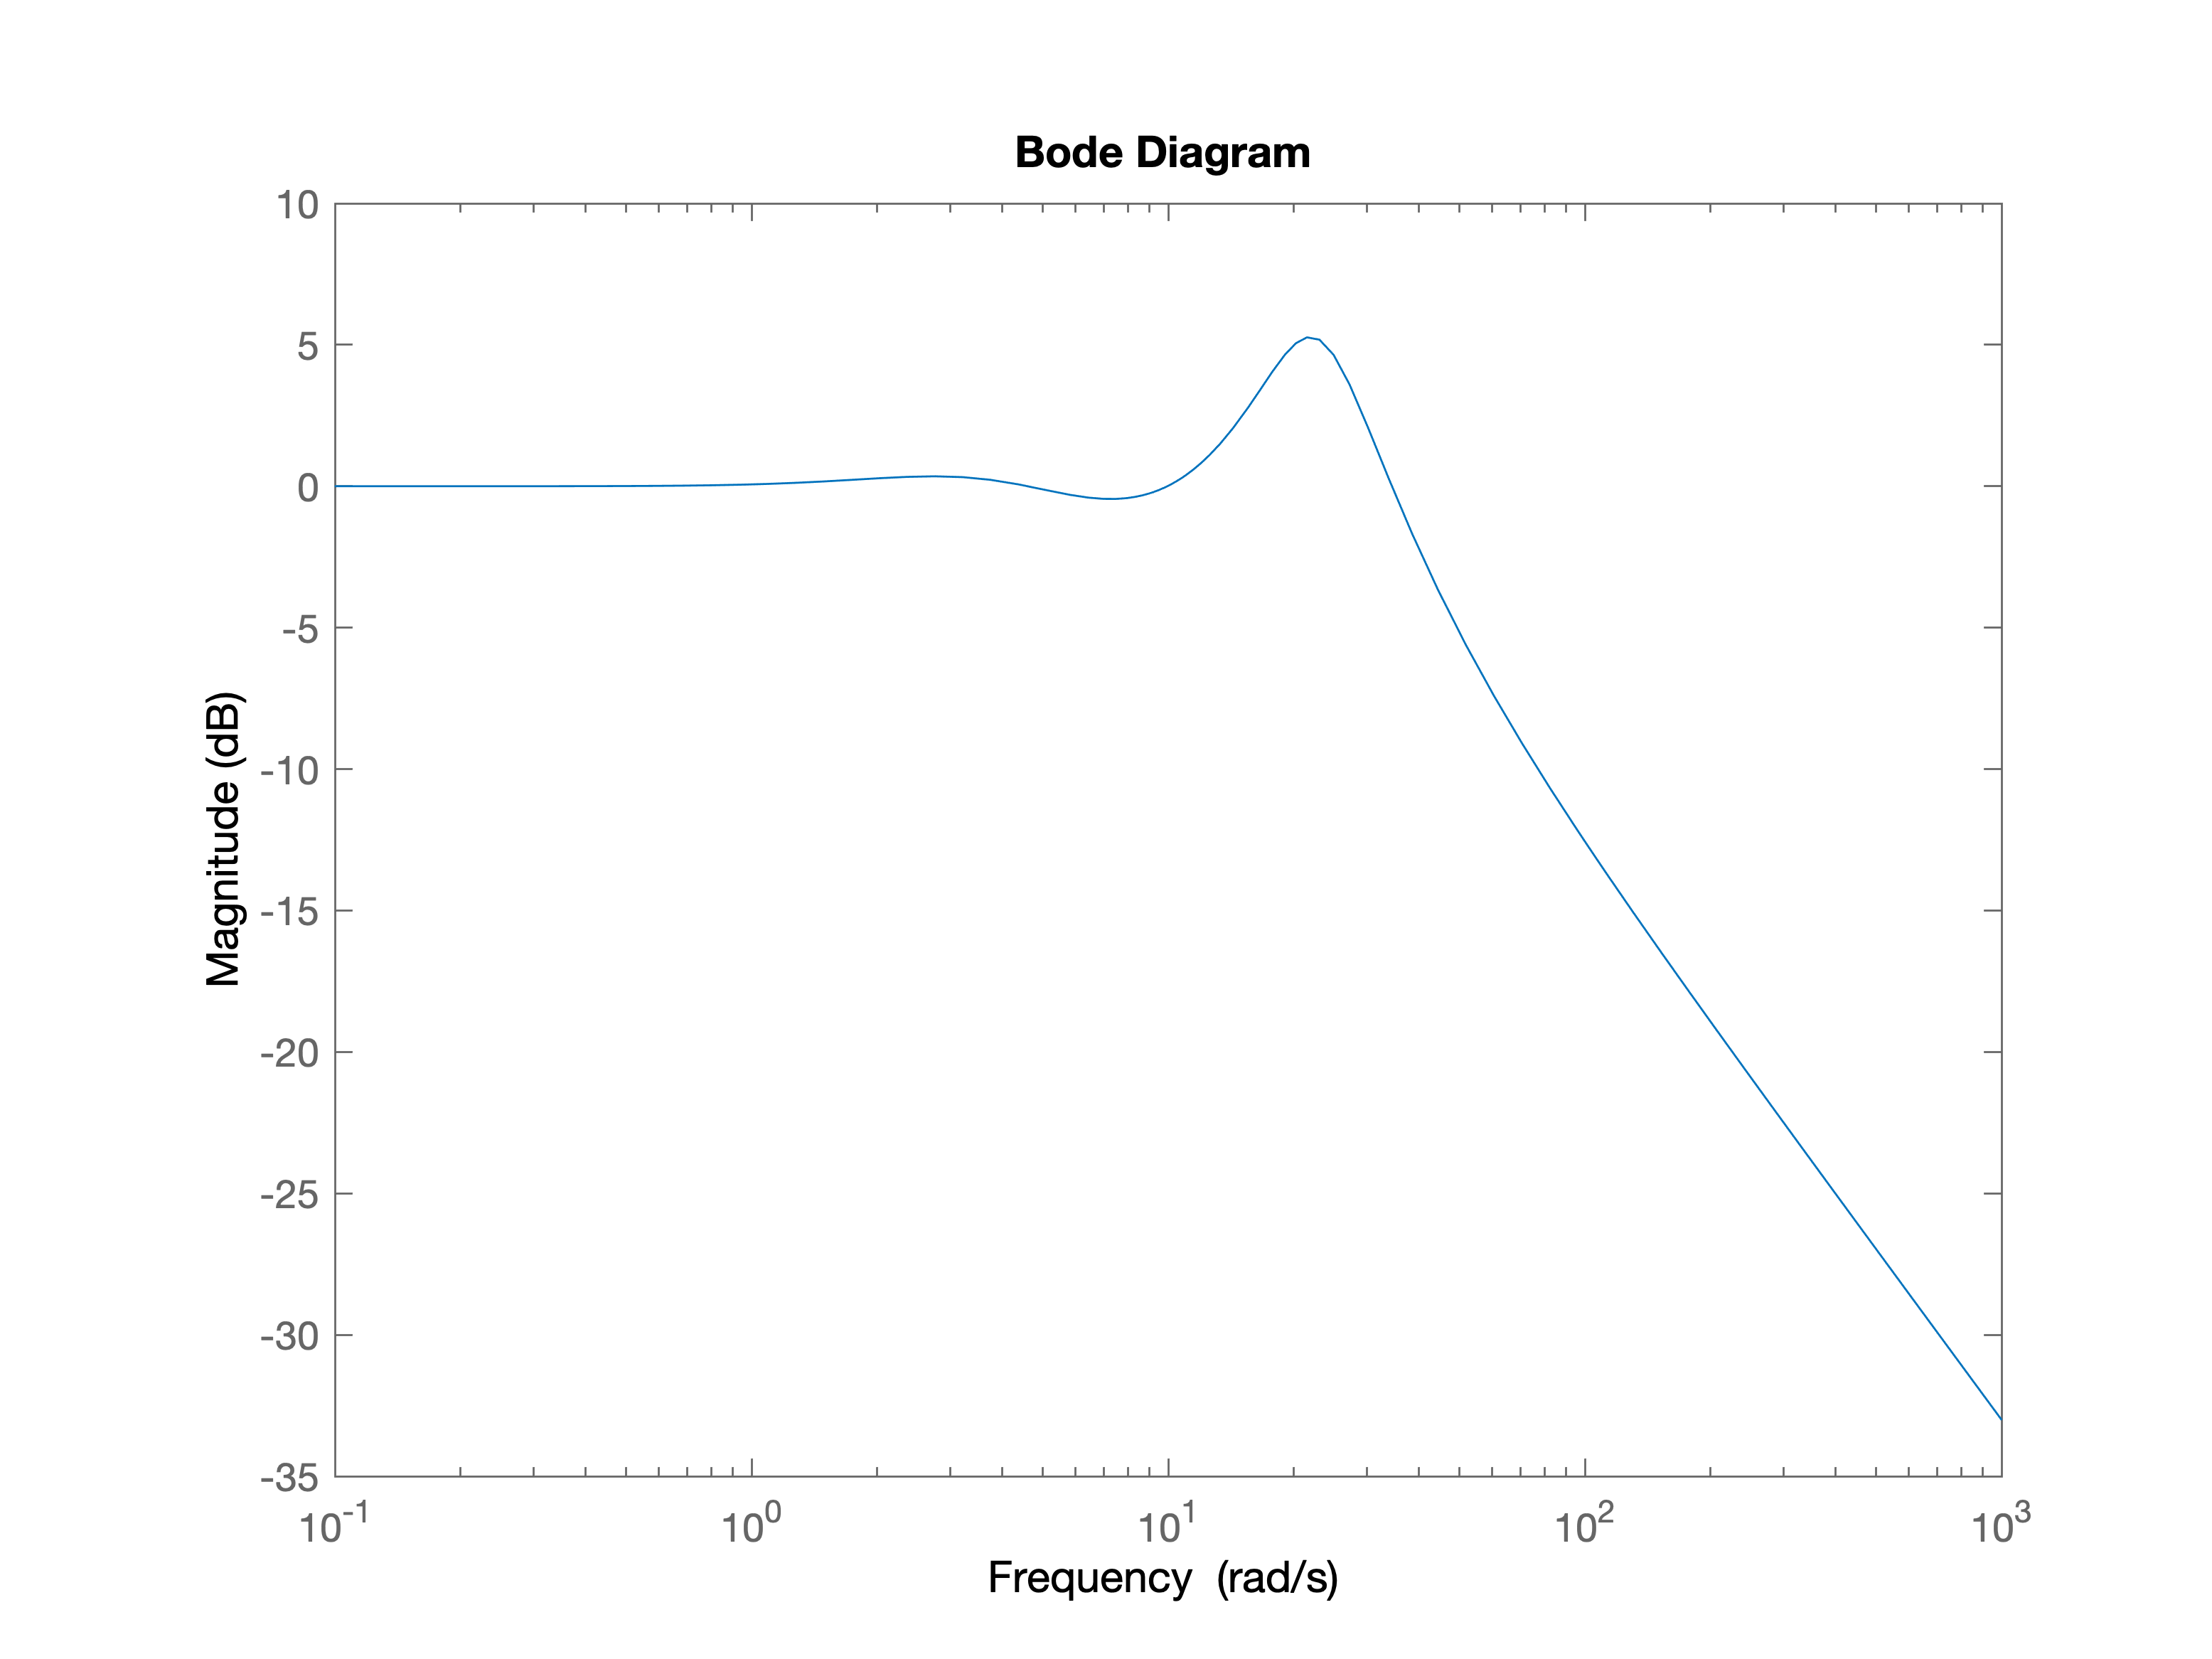
\includegraphics[width=12cm]{../Figure/Q1/Q1_c/bode_n2y.png}
    \end{figure}
    System has a good performance at high frequency but not good performance at low frequency.
\end{itemize}